% !TeX program = xelatex
\documentclass[tikz, border=2pt]{standalone}
\usepackage{ctex}
\usepackage{tikz}
\usetikzlibrary{shadows, positioning, arrows.meta, decorations.pathmorphing, fit, backgrounds, calc}
\begin{document}
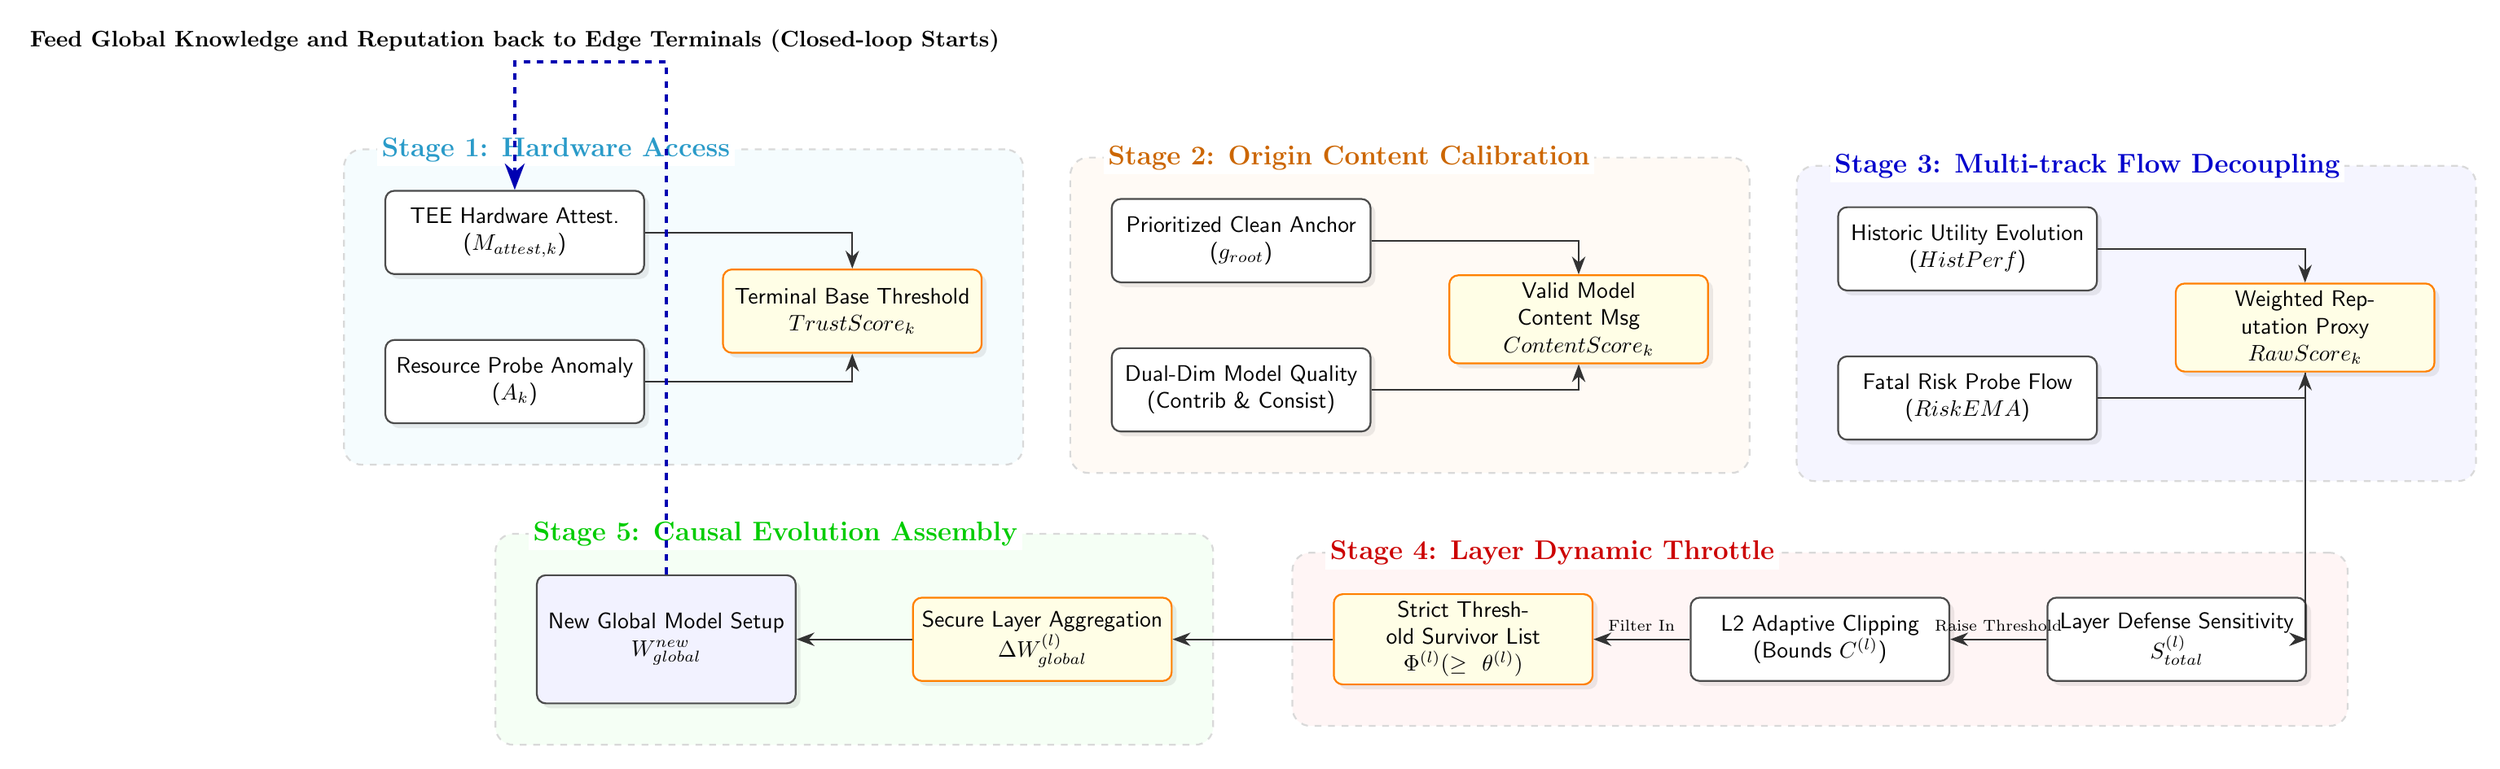
\begin{tikzpicture}[
        font=\sffamily,
        node distance=2.5cm and 2cm,
        % Styles
        phase_bg/.style={draw=gray!30, fill=#1, rounded corners=8pt, inner sep=18pt, dashed, thick},
        block/.style={draw=black!70, fill=white, rounded corners=4pt, text width=3.8cm, align=center, minimum height=1.3cm, thick, drop shadow={opacity=0.15}},
        highlight_block/.style={block, fill=yellow!10, draw=orange, thick},
        arrow/.style={-{Stealth[scale=1.2]}, thick, draw=black!80},
        feedback/.style={-{Stealth[scale=1.2]}, line width=1.5pt, dashed, draw=blue!70!black}
    ]

    % Stage 1 Nodes (Left)
    \node[block] (tee) {TEE Hardware Attest.\\($M_{attest,k}$)};
    \node[block, below=1cm of tee] (anomaly) {Resource Probe Anomaly\\($A_k$)};
    \node[highlight_block, right=1.2cm of anomaly, yshift=1.1cm] (trustscore) {Terminal Base Threshold\\$TrustScore_k$};
    \draw[arrow] (tee) -| (trustscore);
    \draw[arrow] (anomaly) -| (trustscore);

    % Stage 2 Nodes
    \node[block, right=2cm of trustscore, yshift=1.1cm] (groot) {Prioritized Clean Anchor\\($g_{root}$)};
    \node[block, below=1cm of groot] (content) {Dual-Dim Model Quality\\(Contrib \& Consist)};
    \node[highlight_block, right=1.2cm of content, yshift=1.1cm] (contentscore) {Valid Model Content Msg\\$ContentScore_k$};
    \draw[arrow] (groot) -| (contentscore);
    \draw[arrow] (content) -| (contentscore);

    % Stage 3 Nodes
    \node[block, right=2cm of contentscore, yshift=1.1cm] (hist) {Historic Utility Evolution\\($HistPerf$)};
    \node[block, below=1cm of hist] (risk) {Fatal Risk Probe Flow\\($RiskEMA$)};
    \node[highlight_block, right=1.2cm of risk, yshift=1.1cm] (rawscore) {Weighted Reputation Proxy\\$RawScore_k$};
    \draw[arrow] (hist) -| (rawscore);
    \draw[arrow] (risk) -| (rawscore);

    % Stage 4 Nodes (Return flow below)
    \node[block, below=3.5cm of rawscore, xshift=-2cm] (gate) {Layer Defense Sensitivity\\$S_{total}^{(l)}$};
    \node[block, left=1.5cm of gate] (clip) {L2 Adaptive Clipping\\(Bounds $C^{(l)}$)};
    \node[highlight_block, left=1.5cm of clip] (survivor) {Strict Threshold Survivor List\\$\Phi^{(l)} (\ge \theta^{(l)})$};
    \draw[arrow] (rawscore) |- (gate);
    \draw[arrow] (gate) -- node[above, font=\scriptsize] {Raise Threshold} (clip);
    \draw[arrow] (clip) -- node[above, font=\scriptsize] {Filter In} (survivor);

    % Stage 5 Nodes
    \node[highlight_block, left=2.5cm of survivor] (agg) {Secure Layer Aggregation\\$\Delta W_{global}^{(l)}$};
    \node[block, fill=blue!5, left=1.8cm of agg, minimum height=2cm] (global) {New Global Model Setup\\$W_{global}^{new}$};
    \draw[arrow] (survivor) -- (agg);
    \draw[arrow] (agg) -- (global);

    % Closed Loop Feedback
    \draw[feedback] (global.north) |- ([yshift=2.0cm]tee.north) -| node[above, near start, font=\bfseries] {Feed Global Knowledge and Reputation back to Edge Terminals (Closed-loop Starts)} (tee.north);

    % Grouping Backgrounds
    \begin{scope}[on background layer]
        \node[phase_bg=cyan!4, fit=(tee) (anomaly) (trustscore)] (bg1) {};
        \node[font=\bfseries\large, text=cyan!80!black, fill=white, inner sep=2pt] at (bg1.north west) [anchor=south west, xshift=15pt, yshift=-8pt] {Stage 1: Hardware Access};

        \node[phase_bg=orange!4, fit=(groot) (content) (contentscore)] (bg2) {};
        \node[font=\bfseries\large, text=orange!80!black, fill=white, inner sep=2pt] at (bg2.north west) [anchor=south west, xshift=15pt, yshift=-8pt] {Stage 2: Origin Content Calibration};

        \node[phase_bg=blue!4, fit=(hist) (risk) (rawscore)] (bg3) {};
        \node[font=\bfseries\large, text=blue!80!black, fill=white, inner sep=2pt] at (bg3.north west) [anchor=south west, xshift=15pt, yshift=-8pt] {Stage 3: Multi-track Flow Decoupling};

        \node[phase_bg=red!4, fit=(gate) (clip) (survivor)] (bg4) {};
        \node[font=\bfseries\large, text=red!80!black, fill=white, inner sep=2pt] at (bg4.north west) [anchor=south west, xshift=15pt, yshift=-8pt] {Stage 4: Layer Dynamic Throttle};

        \node[phase_bg=green!4, fit=(agg) (global)] (bg5) {};
        \node[font=\bfseries\large, text=green!80!black, fill=white, inner sep=2pt] at (bg5.north west) [anchor=south west, xshift=15pt, yshift=-8pt] {Stage 5: Causal Evolution Assembly};
    \end{scope}
    
    \end{tikzpicture}
\end{document}
